
%%% Local Variables: 
%%% mode: latex
%%% TeX-master: t
%%% End: 

\chapter{角毛藻显微图像特征提取}
\label{cha2}
角毛藻细胞壁表面结构细微并且分布有以不同方式生长的角毛。由于角毛藻的特征主要集中在角毛上,因此在分割角毛藻显微图像过程中,能否将脚毛准确的提取出来起着决定性作用。

图\ref{jiaomaozao}所示为三种常见角毛藻显微图像:
\begin{figure}[h]
  \centering
  \begin{subfigure}{3cm}
    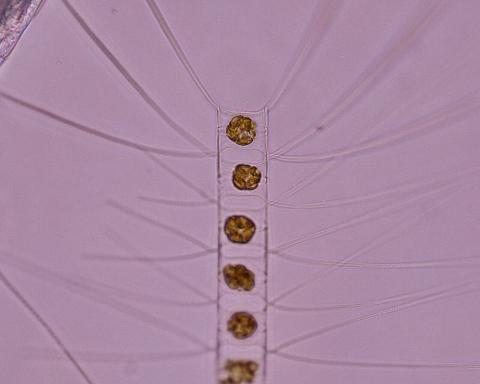
\includegraphics[height=3.5cm]{jiaomaozao1.jpg}
  \end{subfigure}
  \hspace{4em}
  \begin{subfigure}{0.2\textwidth}
    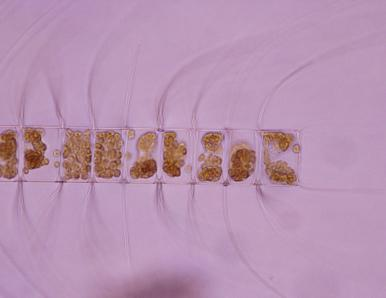
\includegraphics[height=3.5cm]{jiaomaozao2.jpg}
  \end{subfigure}
  \hspace{4em}
  \begin{subfigure}{0.25\textwidth}
    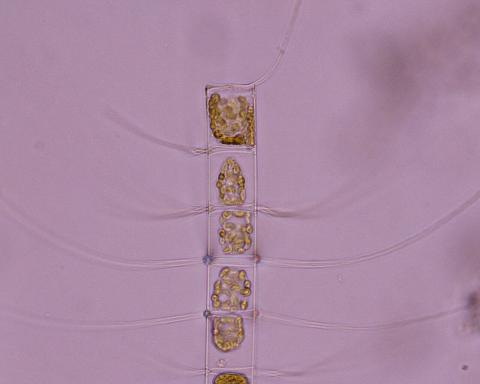
\includegraphics[height=3.5cm]{jiaomaozao3.jpg}
  \end{subfigure}
  \caption{三种常见角毛藻显微图像}
  \label{jiaomaozao}
\end{figure}

通过对图\ref{jiaomaozao}中三种图像的观察,可以发现角毛藻的显微图像具有以下三个特征:
\begin{enumerate}
\item角毛部分长而细,并且其颜色通常与背景十分相近;
\item一些角毛藻显微图像中背景部分含有大量噪声且不易去除;
\item 图像中角毛藻的边缘部分,特别是角毛的边缘部分模糊不清呈条状分布。
\end{enumerate}

为了有效的提取尽可能多的角毛信息,本章运用了一种提取角毛藻角毛特征的基于灰度曲面方向角模型的方法。
\section{灰度曲面方向角模型}
 灰度曲面方向角模型(Grayscale Surface Direction Angle Model)是由中国海洋大学郑海永\cite{zheng2014automatic}等于2014年提出的,基于该模型的从角毛藻显微图像中分割出角毛的算法能够比传统基于边缘或基于区域的分割方法得到更好的分割结果。

一副给定的图像上的每一个像素点都可以确定一个对应的灰度曲面。由于某一点的法向量在大小为的曲面中难以确定,因此采用近似处理来确定法向量。给定一点,首先分别求出该点及其三个相邻像素点构成的四个平面的法向量,再对四个法向量求取平均值来近似表示该点的法向量。灰度曲面方向角模型的具体算法过程如下:
\begin{figure}[ht!]
   \centering
  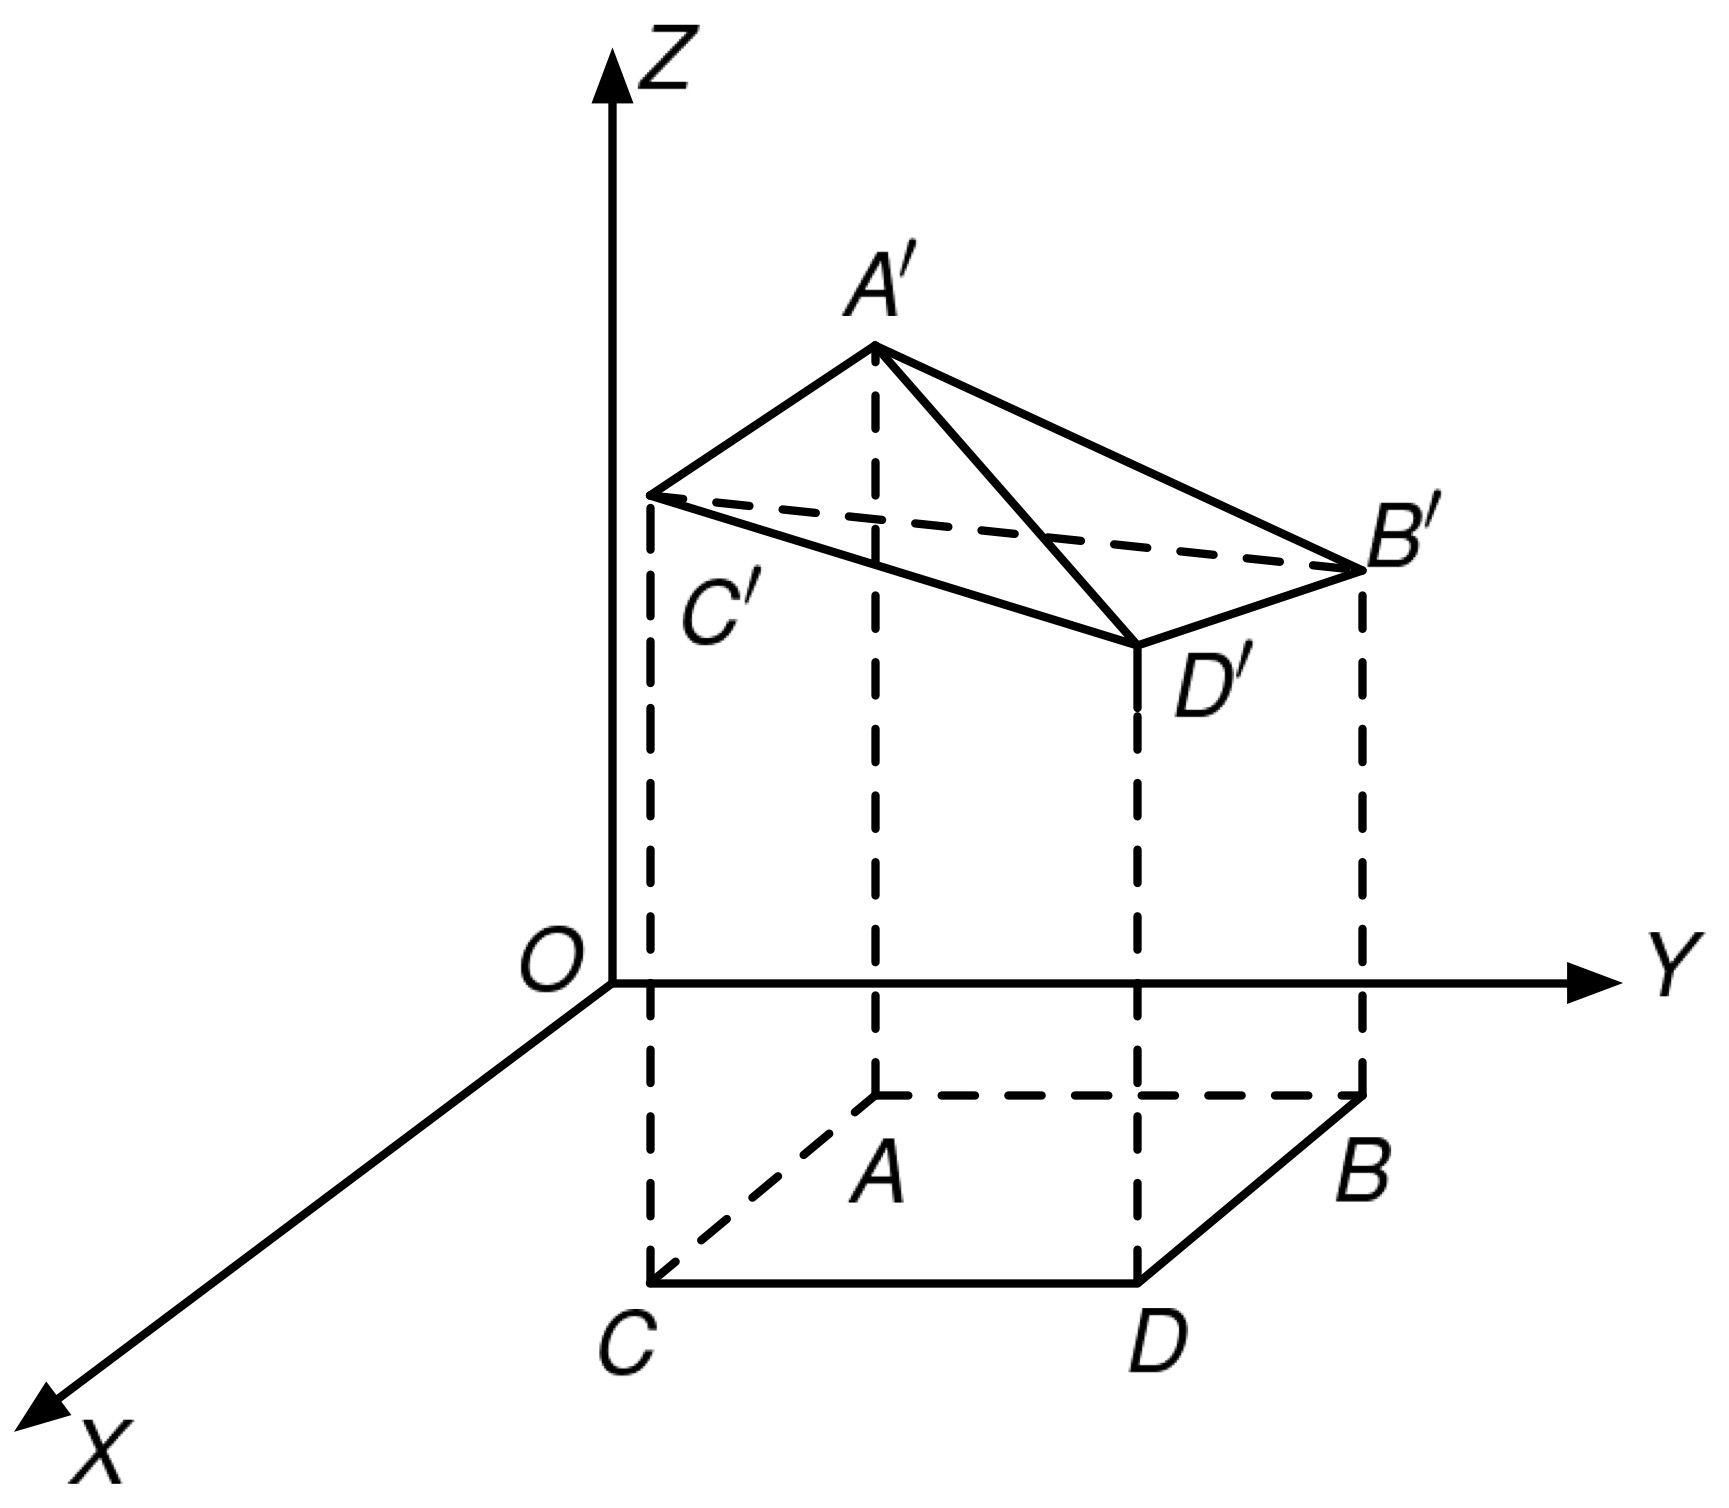
\includegraphics[width=0.8\linewidth]{figure.jpg}
  \caption{}
   \label{GSDAM}
 \end{figure}
 
如图\ref{GSDAM},对整副图片建立空间直角坐标系坐标系,其中$(X,Y)$是像素的空间位置,$Z$是该像素对应的灰度值。对于一个给定的像素点$A$可以确定其位置和灰度值,像素点的三个相邻的像素点分别为$B$、$C$和$D$。在空间直角坐标系中,$A$、$B$、$C$、$D$四个点分别对应$A'$、$B'$、$C'$、$D'$并且这四个点可以形成四个互不重叠的三角形面$A'B'C'$、$A'C'D'$、$A'B'D'$和$B'C'D'$。

以平面$A'B'C'$为例,平面$A'B'C'$的法向量$\overrightarrow{f_{A'B'C'}}$可以通过$\overrightarrow{f_{A'B'C'}}=\overrightarrow{A'C'}\times\overrightarrow{A'B'}$来计算,其中向量$\overrightarrow{A'C'}=(1,0,I(i+1,j)-I(i,j))$ ,向量$\overrightarrow{A'B'}=(0,1,I(i,j+1)-I(i,j))$。使用同样的方法分别计算出其余平面的法向量$\overrightarrow{f_{A'C'D'}}$、$\overrightarrow{f_{A'B'D'}}$、$\overrightarrow{f_{B'C'D'}}$,则可以利用四个三角形面的法向量近似得到的法向量:
\begin{equation}
\overrightarrow{f_{A'}}=(\overrightarrow{f_{A'B'C'}}+\overrightarrow{f_{A'C'D'}}+\overrightarrow{f_{A'B'D'}}+\overrightarrow{f_{B'C'D'}})/4
\end{equation}
通过$A'$的法向量$\overrightarrow{f_{A'}}$,可以计算出该法向量与空间直角坐标系三个坐标轴之间的夹角如下:
\begin{equation}
\begin{split}
\theta_{x}(i,j)=360\times \cos ^{-1}(f_{x}/|\overrightarrow {f_{A'}}| )/2\pi\\
\theta_{y}(i,j)=360\times \cos ^{-1}(f_{y}/|\overrightarrow {f_{A'}}| )/2\pi\\
\theta_{z}(i,j)=360\times \cos ^{-1}(f_{z}/|\overrightarrow {f_{A'}}| )/2\pi
\end{split}
\end{equation}
其中$f_{x}$、$f_{y}$、$f_{z}$分别是$\overrightarrow{f_{A'}}$在轴$X$、$Y$、$Z$的坐标值,$|\overrightarrow {f_{A'}}|$是$\overrightarrow{f_{A'}}$的模。
依次对范围在$[\min(\theta),\max(\theta)]$的三个夹角$\theta_{x}$、$\theta_{y}$、$\theta_{z}$进行灰度映射,映射后其范围在$[0,255]$之间:
\begin{equation}
\begin{split}
Map_{x}(i,j)=255\times\frac{\theta_{x}(i,j)-\min(\theta_{x})}{\max(\theta_{x})-\min(\theta_{x})}\\
Map_{y}(i,j)=255\times\frac{\theta_{y}(i,j)-\min(\theta_{y})}{\max(\theta_{y})-\min(\theta_{y})}\\
Map_{z}(i,j)=255\times\frac{\theta_{z}(i,j)-\min(\theta_{z})}{\max(\theta_{z})-\min(\theta_{z})}
\end{split}
\end{equation}
此外还可以得到$xz$平面和$yz$平面的灰度映射:
\begin{equation}
\begin{split}
Map_{xz}(i,j)=\sqrt{Map_{x}(i,j)^{2}+Map_{z}(i,j)^{2}}\\
Map_{yz}(i,j)=\sqrt{Map_{y}(i,j)^{2}+Map_{z}(i,j)^{2}}
\end{split}
\end{equation}
利用同样的方法来处理图像中的所有像素可以得到五张灰度图像$Map_{x}$、$Map_{y}$、$Map_{z}$、$Map_{xz}$、$Map_{yz}$,对于图像右侧和下侧边缘部分的像素,可以采取重复边缘灰度值的方式来扩展图像边缘。
\section{实验结果}
\subsection{实验前的预处理操作}
由于选取的数据集中原始彩色角毛藻图像的尺寸非常大,在后续SVM训练和预测过程中运算复杂度很高、耗时较长,因此为了降低运算复杂度并减少运算时间,将角毛藻显微图像调整至原来尺寸的0.15倍。

此外,考虑到显微图像的颜色会因成像设备和滤波器的不同而产生差异,在实验开始前需要将原始调整后的RGB显微图像转化成灰度图像。此时,每一幅灰度图像都可以视为一个空间直角坐标系。
\begin{figure}[ht!]
\centering
\begin{minipage}[b]{0.45\linewidth} 
      \centering 
      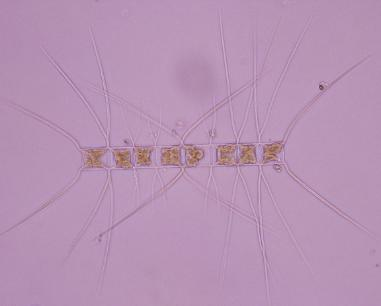
\includegraphics[width=0.9\linewidth]{resize.jpg}
        \centerline{(a) 原始显微图像}\medskip
\end{minipage}
  \begin{minipage}[b]{0.45\linewidth}
    \centering
    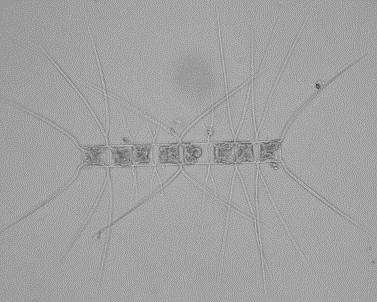
\includegraphics[width=0.9\linewidth]{resize_gray.jpg}
      \centerline{(b) 调整后灰度图像}\medskip
  \end{minipage}
 \caption{实验前的预处理操作}
\end{figure}

\subsection{角毛藻显微图像特征提取结果}
对每一幅原始灰度图像中的所有像素使用灰度平面方向角模型方法进行处理操作可以得到五张含有角毛藻目标细胞和角毛特征信息的灰度映射图像,这五副灰度图可以用作后续支持向量机分类器的输入特征。

如图\ref{GSDAMresults}所示为并基角毛藻显微图像的特征提取结果:

\begin{figure}[ht!]
\centering
    \begin{minipage}[b]{0.45\linewidth}
    \centering
    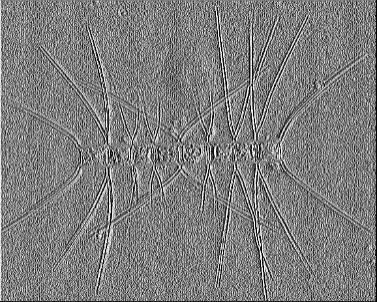
\includegraphics[width=0.9\linewidth]{mapx.jpg}
      \centerline{(a) x方向灰度映射图}\medskip
  \end{minipage}
  \begin{minipage}[b]{0.45\linewidth}
    \centering
    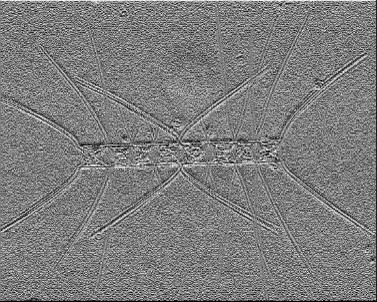
\includegraphics[width=0.9\linewidth]{mapy.jpg}
      \centerline{(b) y方向灰度映射图}\medskip
  \end{minipage}
   \begin{minipage}[b]{0.45\linewidth}
    \centering
    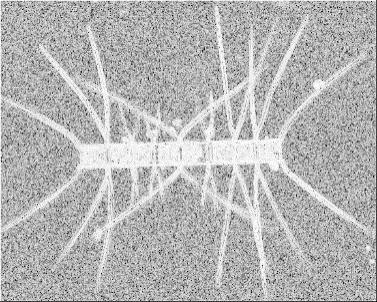
\includegraphics[width=0.9\linewidth]{mapz.jpg}
      \centerline{(c) z方向灰度映射图}\medskip
  \end{minipage}
  \begin{minipage}[b]{0.45\linewidth}
    \centering
    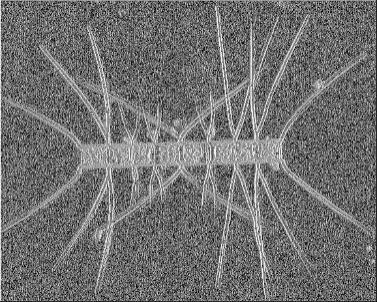
\includegraphics[width=0.9\linewidth]{mapxz.jpg}
      \centerline{(d) xz方向灰度映射图}\medskip
  \end{minipage}
   \begin{minipage}[b]{0.45\linewidth}
    \centering
    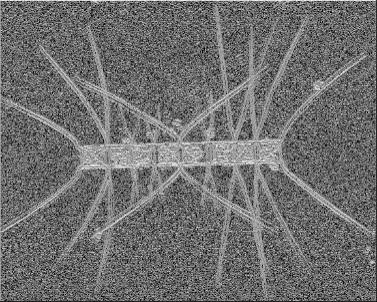
\includegraphics[width=0.9\linewidth]{mapyz.jpg}
      \centerline{(e) yz方向灰度映射图}\medskip
  \end{minipage}
 \caption{角毛藻显微图像的特征提取结果}
  \label{GSDAMresults}
\end{figure}


\section{本章小结}
本章针对角毛藻独特的生物形态学特征,使用灰度曲面方向角模型对角毛藻显微图像进行特征提取。

首先介绍了灰度曲面方向角模型的基本原理,然后通过实验验证了采用灰度平面方向角模型的特征提取方法能够较为准确的提取出角毛等特征信息,有助于后续操作中利用连通区域预分割产生支持向量机的训练样本,并且可以作为支持向量机的输入特征。

